\documentclass{beamer}
\usepackage{tikz}
\usepackage{amsmath}
\usepackage{algorithm}
\usepackage{algorithmic}

\definecolor{usccardinal}{rgb}{0.6, 0.0, 0.0}
\definecolor{tropicalrainforest}{rgb}{0.0, 0.46, 0.37}

\usetikzlibrary{shapes,arrows,positioning,calc}
\usetheme{metropolis}
\setbeamercolor{background canvas}{bg=white}

\title{Toward Controlled Generation of Text}
\date{}
\author{Hu, Yang, Liang, Salakhutdinov \& Xing}
\institute{ICML 2017}

\begin{document}
\maketitle

\section{Motivation}

\begin{frame}{Motivation}
	\centering
	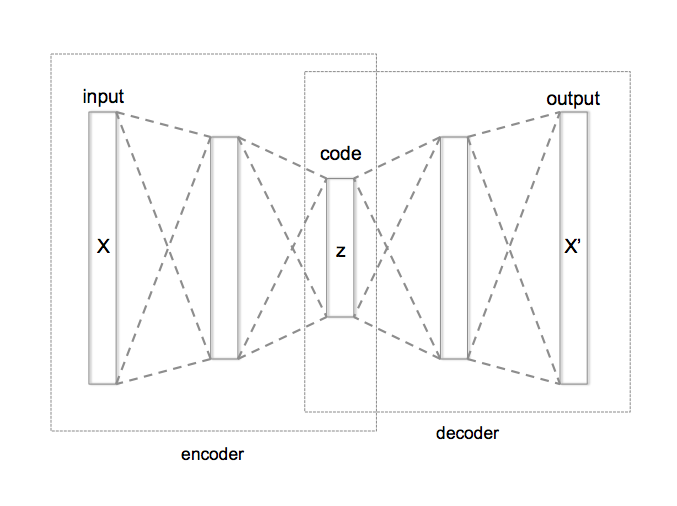
\includegraphics[width=.9\textwidth]{images/autoencoder.png}
	{\tiny \footnote{https://commons.wikimedia.org/wiki/File:Autoencoder\_structure.png}}
\end{frame}

\begin{frame}{Motivation}
	\centering
	{\Large Distentangled Latent Representations} \\
	\vspace{1cm}
	\begin{columns}[T] % align columns
		\begin{column}{.3\textwidth}
			\centering
			\begin{tabular}{ c c }
				I love this movie & $\rightarrow$ \\
				I hate this movie & $\rightarrow$ \\
			\end{tabular} \\
			\vspace{1.8cm}
			{\color{white} \begin{tabular}{ c c }
					I love this movie & $\rightarrow$ \\
					I hate this movie & $\rightarrow$ \\
				\end{tabular}}
		\end{column}
		\hfill
		\begin{column}{.6\textwidth}
			\centering
			\begin{tabular}{ | c | c | c | c | }
				\hline
				$0.21$ & $0.32$ & $0.74$ & $0.43$ \\
				\hline
				\hline
				$0.45$ & $0.78$ & $0.97$ & $0.17$ \\
				\hline
			\end{tabular}
			{\color{white}{\Huge$$\Downarrow$$}
			\begin{tabular}{ | c | c | c | c | }
				\hline
				$0.68$ & $0.12$ & $0.33$ & $1.00$ \\
				\hline
				\hline
				$0.68$ & $0.12$ & $0.33$ & $0.00$ \\
				\hline
			\end{tabular}}
		\end{column}
	\end{columns}
\end{frame}

\begin{frame}{Motivation}
	\centering
	{\Large Distentangled Latent Representations} \\
	\vspace{1cm}
	\begin{columns}[T] % align columns
		\begin{column}{.3\textwidth}
			\centering
			\begin{tabular}{ c c }
				I love this movie & $\rightarrow$ \\
				I hate this movie & $\rightarrow$ \\
			\end{tabular}\\
			\vspace{1.8cm}
			\begin{tabular}{ c c }
				I love this movie & $\rightarrow$ \\
				I hate this movie & $\rightarrow$ \\
			\end{tabular}
		\end{column}
		\hfill
		\begin{column}{.6\textwidth}
			\centering
			\begin{tabular}{ | c | c | c | c | }
				\hline
				$0.21$ & $0.32$ & $0.74$ & $0.43$ \\
				\hline
				\hline
				$0.45$ & $0.78$ & $0.97$ & $0.17$ \\
				\hline
			\end{tabular}
			{\Huge$$\Downarrow$$}
			\begin{tabular}{ | c | c | c | c | }
				\hline
				$0.68$ & $0.12$ & $0.33$ & {\color{red}$1.00$} \\
				\hline
				\hline
				$0.68$ & $0.12$ & $0.33$ & {\color{red}$0.00$} \\
				\hline
			\end{tabular}
		\end{column}
	\end{columns}
\end{frame}


\begin{frame}{Motivation}
	\centering
	{\Huge Problem Statement} \\
	\vspace{1cm}
	{\Large Generate fake samples similar to the source distribution by conditioning their generation on a tunable set of attributes.}
\end{frame}


\section{Method}
\begin{frame}{Notation}
	\large
	\begin{tabular}{ l c l }
		$x$       & $\Rightarrow$ & \textbf{source corpus}                                                 \\
		$\hat{x}$ & $\Rightarrow$ & \textbf{output corpus}                                                 \\
		$c$       & $\Rightarrow$ & \textbf{structured code}, known label for each document                \\
		$z$       & $\Rightarrow$ & \textbf{unstructured latent code}                                      \\
		\\
		$E$       & $\Rightarrow$ & \textbf{encoder}, parameterized to generate $z$                        \\
		$G$       & $\Rightarrow$ & \textbf{decoder/generator}, produces $\hat{x}$ conditioned on $(z, c)$ \\
		$D$       & $\Rightarrow$ & \textbf{discriminator}, predicts $c$ given $\hat{x}$.                  \\
		$\tau$    & $\Rightarrow$ & \textbf{softmax temperature}, for decoder word prediction              \\
	\end{tabular}
\end{frame}

\begin{frame}{Architecture}
	\tikzstyle{block} = [draw, rectangle, minimum height=2em]
	\centering
	\begin{tikzpicture}[auto, node distance=1cm,>=latex']
		\node [label={[distance=0.05cm]270:\tiny{input-text}}, block] (input) {$x$};
		\node [label={[distance=0.05cm]270:\tiny{encoder}}, purple, block, right = of input] (encoder) {$E$};
		\node [label={[distance=0.05cm]270:\tiny{latent-code}}, block, right = of encoder] (latent) {$z$};
		\node [label={[distance=0.05cm]270:\tiny{structured-code}}, block, below = of latent] (code) {$c$};
		\node [label={[distance=0.05cm]270:\tiny{generator}}, block, right = of latent] (generator) {$G(z, c)$};
		\node [label={[distance=0.05cm]0:\tiny{output}}, block, right = of generator] (output) {$\hat{x}$};
		\node [coordinate, above = of output] (inter1) {};
		\node [label={[distance=0.05cm]270:\tiny{discriminator}}, block, below = of output] (discriminator) {$D(c|\hat{x})$};

		\draw [->] (input) -- (encoder);
		\draw [->] (encoder) -- (latent);
		\draw [->] (latent) -- (generator);
		\draw [->] (code) -- (generator);
		\draw [->] (generator) -- (output);
		\draw [-] (output) -- (inter1);
		\draw [->] (inter1) -| (encoder);
		\draw [->] (output) -- (discriminator);

		% Independency constraint
		\draw [magenta, dashed, ->] ($(inter1) + (-0.15,-0.15)$) -- ($(output) + (-0.15,0.45)$) node[label={[label distance=0.01cm]110:\tiny{$\mathcal{L}_{attr}$}}] {};
		\draw [red, dashed, ->] ($(output) + (-0.25,0.15)$) -- ($(generator) + (0.7,0.15)$) node[label={[label distance=0.01cm]10:\tiny{$\mathcal{L}_{rec}$}}] {};

		% Discriminator loss
		\draw [blue, dashed, ->] ($(discriminator) + (-0.15,0.45)$) -- ($(output) + (-0.15,-0.45)$) node[label={[label distance=0.01cm]250:\tiny{$\mathcal{L}_{adv}$}}] {};
	\end{tikzpicture}
\end{frame}

\begin{frame}{Unrolled Architecture}
	\tikzstyle{block} = [draw, rectangle, minimum height=2em]
	\centering
	\begin{tikzpicture}[auto, node distance=1cm,>=latex']
		\node [label={[distance=0.05cm]90:\tiny{input-text}}, block] (input) {$x$};
		\node [label={[distance=0.05cm]90:\tiny{encoder}}, purple, block, right = of input] (encoder1) {$E$};
		\node [label={[distance=0.05cm]90:\tiny{latent-code}}, block, right = of encoder1] (latent1) {$z$};
		\node [label={[distance=0.05cm]270:\tiny{structured-code}}, block, below = of latent1] (code) {$c$};
		\node [label={[distance=0.05cm]90:\tiny{generator}}, block, right = of latent1] (generator) {$G(z, c)$};
		\node [label={[distance=0.05cm]90:\tiny{output}}, block, right = of generator] (output) {$\hat{x}$};
		\node [label={[distance=0.05cm]270:\tiny{discriminator}}, block, below = of output] (discriminator) {$D(c|\hat{x})$};
		\node [label={[distance=0.05cm]90:\tiny{encoder}}, purple, block, right = of output] (encoder2) {$E$};
		\node [label={[distance=0.05cm]90:\tiny{latent-code}}, block, right = of encoder2] (latent2) {$\hat{z}$};

		\draw [->] (input) -- (encoder1);
		\draw [->] (encoder1) -- (latent1);
		\draw [->] (latent1) -- (generator);
		\draw [->] (code) -- (generator);
		\draw [->] (generator) -- (output);
		\draw [->] (output) -- (discriminator);
		\draw [->] (output) -- (encoder2);
		\draw [->] (encoder2) -- (latent2);

		% Independency constraint
		\draw [magenta, dashed, ->] ($(encoder2) + (-0.4,0.15)$) -- ($(output) + (0.25,0.15)$) node[label={[label distance=0.01cm]10:\tiny{$\mathcal{L}_{attr}$}}] {};
		\draw [red, dashed, ->] ($(output) + (-0.25,0.15)$) -- ($(generator) + (0.7,0.15)$)node[label={[label distance=0.01cm]10:\tiny{$\mathcal{L}_{rec}$}}] {};

		% Discriminator loss
		\draw [blue, dashed, ->] ($(discriminator) + (-0.15,0.45)$) -- ($(output) + (-0.15,-0.45)$) node[label={[label distance=0.01cm]260:\tiny{$\mathcal{L}_{adv}$}}] {};
	\end{tikzpicture}
\end{frame}

\begin{frame}{Optimization Objectives}
	\textbf{Discriminator Optimization}

	\begin{itemize}
		\item Maximize the likelihood of predicting the correct distribution of the structured code $c$ given the labeled examples $X_L$.
		      \begin{equation*}
			      \mathcal{L}_s(\theta_D) = - \mathbb{E}_{X_L}[log q_D(c_L|x_L)]
		      \end{equation*}
		\item Maximize the likelihood of predicting the correct distribution of the structured code $c$ given the generated sentences $\hat{x}$. Also minimize the empirically observed Shannon entropy of the discriminator predictions $q_D(c'|\hat{x})$.
		      \begin{equation*}
			      \mathcal{L}_u(\theta_D) = - \mathbb{E}_{p_G(\hat{x}|z,c)p(z)p(c)}
			      [log q_D(c|\hat{x}) + \beta \mathcal{H}(q_D(c'|\hat{x}))]
		      \end{equation*}
	\end{itemize}
\end{frame}

\begin{frame}{Optimization Objectives}
	\textbf{Generator Optimization}

	\begin{itemize}
		\item Maximize the likelihood of predicting the original document $x$, given the latent spaces and the generator $G(z,c)$.
		      \begin{eqnarray*}
			      \mathcal{L}_{VAE}(\theta_G, \theta_E; x) &=&
			      - \mathbb{E}_{q_E(z|x)q_D(c|x)}[log p_G(x|z,c)] \\ & &
			      + KL(q_E(z|x)||p(z))
		      \end{eqnarray*}
		\item Maximize the likelihood of generating the output documents with the correct structured code $c$
		      \begin{equation*}
			      \mathcal{L}_{attr, c}(\theta_G) = - \mathbb{E}_{p(z)p(c)}
			      [log q_D(c|\tilde{G_{\tau}}(z,c))]
		      \end{equation*}
	\end{itemize}
\end{frame}

\begin{frame}{Training Objectives}
	\textbf{Additional Generator Optimization: Independency Constraint}

	The encoder is re-used to regenerate the latent distribution $z$ devoid of the structured code $c$, from the output distribution $\tilde{G_{\tau}}(z,c)$.
	\begin{equation*}
		\mathcal{L}_{attr, z}(\theta_G) = - \mathbb{E}_{p(z)p(c)}
		[log q_E(z|\tilde{G_{\tau}}(z,c))]
	\end{equation*}
\end{frame}

\begin{frame}{Training Objectives}

	\textbf{Generator:}
	\begin{eqnarray*}
		\operatorname*{min}_{\theta_G} \mathcal{L}_G =
		& \mathcal{L}_{VAE} & \text{(reconstruction loss)} \\
		& + \lambda_c \mathcal{L}_{attr,c} & \text{(style entanglement)} \\
		& + \lambda_z \mathcal{L}_{attr,z} & \text{(independency constraint)}
	\end{eqnarray*}

	\textbf{Discriminator:}
	\begin{eqnarray*}
		\operatorname*{min}_{\theta_D} \mathcal{L}_D =
		& \mathcal{L}_{s} & \text{(labeled example classification)} \\
		& + \lambda_u \mathcal{L}_{attr,u} & \text{(synthesized example classification)}
	\end{eqnarray*}
\end{frame}

\begin{frame}{Algorithm}
	\begin{algorithm}[H]
		\centering
		\begin{algorithmic}[1]
			\REQUIRE A large corpus of unlabeled sentences $\mathcal{X}=\{x\}$ \\
			\quad A few sentence attribute labels $\mathcal{X}_L = \{(x_L,c_L)\}$ \\
			\quad Parameters: $\lambda_c, \lambda_z, \lambda_u, \beta$  -- balancing parameters \\
			\STATE Initialize the base VAE by minimizing $\mathcal{L}_{VAE}$ on $\mathcal{X}$
			\REPEAT
			\STATE Train the discriminator $D$ by minimizing $\mathcal{L}_u$
			\STATE Train the generator $G$ and the encoder $E$ by minimizing $\mathcal{L}_G$ and $\mathcal{L}_{VAE}$, respectively.
			\UNTIL{convergence}
			\ENSURE Sentence generator $G$ conditioned on disentangled representation $(z,c)$
		\end{algorithmic}
	\end{algorithm}
\end{frame}

\begin{frame}{Algorithm}
	\centering
	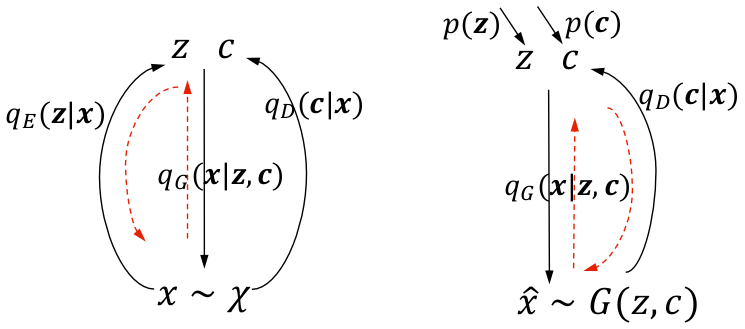
\includegraphics[width=\textwidth]{images/wake-sleep.png}
\end{frame}

\section{Experiments}
\begin{frame}{Experiments}
	\textbf{Simple Reconstruction}
	\begin{itemize}
		\item $350K$ IMDB movie reviews
		\item Sentence length $\leq 15$;
		\item Total sentence count $= 1.4M$
		\item Vocab size $= 16K$
	\end{itemize}
\end{frame}

\begin{frame}{Experiments}

	\textbf{Binary Sentiment Classification and Conditioned Generation}

	\begin{itemize}
		\item \textbf{Stanford Sentiment Treebank-2}: Movie reviews
		      \begin{itemize}
			      \item $2837$ training examples
			      \item Sentence length $\leq 15$
		      \end{itemize}
		\item \textbf{Sentiment Lexicon}: Words used as sentences
		      \begin{itemize}
			      \item $2700$ words
			      \item Sentence length $\leq 15$
		      \end{itemize}
		\item \textbf{IMDB}: Movie reviews
		      \begin{itemize}
			      \item $16K$ training examples
		      \end{itemize}
	\end{itemize}
\end{frame}

\begin{frame}{Experiments}
	\textbf{Tense Classification and Conditioned Generation}
	\begin{itemize}
		\item TimeBank\footnote{http://timeml.org} Lexicon
		\item 5250 words and phrases labeled with one of {“past”, “present”, “future”}
		\item Verbs in different tenses (e.g., “was”, “will be”) as well as time expressions (e.g., “in the future”)
	\end{itemize}
\end{frame}

\begin{frame}{Experiments}
	\textbf{Parameters}
	\begin{itemize}
		\item The generator and encoder are set as single-layer LSTM RNNs with input/hidden dimension of 300 and max decoding time-step count of 15
		\item Discriminators are set as Convolutional Nets
		\item VAE KL-Divergence weight linearly annealed from 0 to 1 during training
		\item Softmax temperature $\tau$ annealed from 1 to 0
		\item Balancing $\lambda$ weights all set to 0.1, $\beta$ is selected on the dev set
	\end{itemize}
\end{frame}

\section{Results}
\begin{frame}{Results}
	\centering
	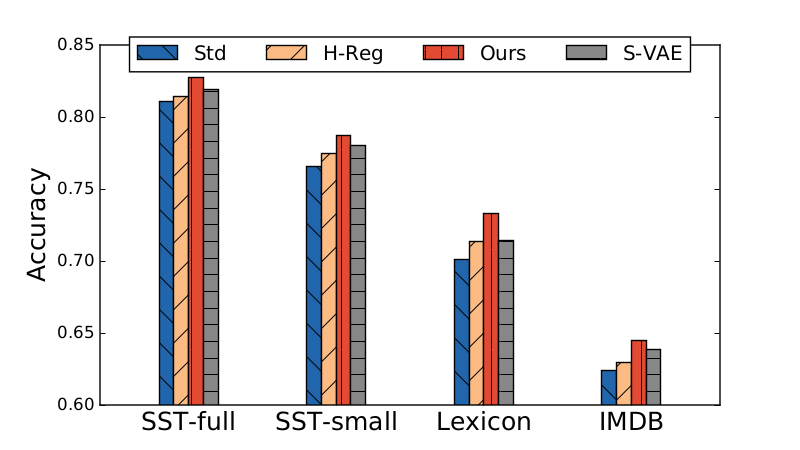
\includegraphics[width=\textwidth]{images/senti.png}
\end{frame}

\begin{frame}{Results}
	\centering
	{\large \textbf{Without `Independency Constraint'}} \\
	\vspace{1cm}
	\small
	\begin{tabular}{ p{.4\linewidth} p{.05\linewidth} p{.4\linewidth} }
		the acting is bad                                      & $\Rightarrow$ & the movie is so much fun                                     \\ \\
		none of this is very original                          & $\Rightarrow$ & highly recommended viewing for its courage , and ideas       \\ \\
		too bland                                              & $\Rightarrow$ & highly watchable                                             \\ \\
		i can analyze this movie without more than three words & $\Rightarrow$ & i highly recommend this film to anyone who appreciates music
	\end{tabular}
\end{frame}

\begin{frame}{Results}
	\centering
	{\large \textbf{With `Independency Constraint'}} \\
	\vspace{1cm}
	\small
	\begin{tabular}{ p{.4\linewidth} p{.05\linewidth} p{.4\linewidth} }
		the film is strictly routine                         & $\Rightarrow$ & the film is full of imagination     \\  \\
		after watching this movie , i felt that disappointed & $\Rightarrow$ & after seeing this film , i 'm a fan \\  \\
		the acting is uniformly bad either                   & $\Rightarrow$ & the performances are uniformly good \\  \\
		this is just awful                                   & $\Rightarrow$ & this is pure genius
	\end{tabular}
\end{frame}

\section{Commentary}
\begin{frame}{Commentary}
	\begin{columns}[T] % align columns
		\begin{column}{.48\textwidth}
			\color{tropicalrainforest}\rule{\linewidth}{4pt}
			\begin{itemize}
				\item Non-parallel attribute-controlled generation
				\item Encoder independency constraint
			\end{itemize}
		\end{column}
		\hfill
		\begin{column}{.48\textwidth}
			\color{usccardinal}\rule{\linewidth}{4pt}
			\begin{itemize}
				\item Constraints don't explicitly provide disentanglement
				\item Susceptible to style bypassing
			\end{itemize}
		\end{column}
	\end{columns}
\end{frame}

\begin{frame}{Related Work}
	\begin{itemize}
		\item Shen, Tianxiao, et al. `Style transfer from non-parallel text by cross-alignment.' Advances in Neural Information Processing Systems. 2017.
		\item Kim, Yoon, et al. `Adversarially regularized autoencoders for generating discrete structures.' arXiv preprint arXiv:1706.04223 (2017).
		\item Fu, Zhenxin, et al. `Style Transfer in Text: Exploration and Evaluation.' arXiv preprint arXiv:1711.06861 (2017).
		\item Melnyk, Igor, et al. `Improved Neural Text Attribute Transfer with Non-parallel Data.' arXiv preprint arXiv:1711.09395 (2017).
	\end{itemize}
\end{frame}

\begin{frame}
	\centering
	\Huge{Questions?}
\end{frame}

\end{document}
